\chapter{The effect of viscosity on the Kelvin-Helmholtz instability in the fan plane of a null point}
\label{chp:null_point_khi}

\graphicspath{{images/null_point_khi/}}

\section{Introduction}

Null points are locations in a magnetic field where the field strength goes to zero and are an abundant feature in the topologically complex coronal magnetic field~\cite{edwardsNullPointDistribution2015}. Given they are sites coinciding with changes in topology, they are strongly associated with reconnection processes~\cite{yangImagingSpectralStudy2020,sunHOTSPINELOOPS2013}. As a result, they are inferred to participate in a number of high-energy phenomena such as in the generation of flare ribbons in compact solar flares~\cite{massonNATUREFLARERIBBONS2009,pontinWhyAreFlare2016a}, production of jets~\cite{moreno-insertisPLASMAJETSERUPTIONS2013} and of coronal mass ejections (CMEs)~\cite{barnesRelationshipCoronalMagnetic2007,zouContinuousNullPointMagnetic2020}, particularly through their involvement in the breakout model of eruptive solar flares~\cite{macleanTopologicalAnalysisMagnetic2005}.

One way in which null point reconnection is known to occur is during the process of null point collapse, where a strong current sheet forms in the vicinity of the null point and enables efficient reconnection between the magnetic field making up the spine and fan plane~\cite{thurgoodImplosiveCollapseMagnetic2018}. This process has the potential to develop into oscillatory reconnection~\cite{thurgoodThreedimensionalOscillatoryMagnetic2017}. It has also been found that twisting the spines of a null point can produce current-vortex sheets in the fan plane which are susceptible to breakup via the Kelvin-Helmholtz instability (KHI)~\cite{wyperKelvinHelmholtzInstabilityCurrentvortex2013}. The KHI has been well studied in MHD~\cite{chandrasekharHydrodynamicHydromagneticStability1981,einaudiResistiveInstabilitiesFlowing1986} and is known to enhance magnetic reconnection in a number of astrophysical contexts~\cite{minEffectsMagneticReconnection1997,kowalKelvinHelmholtzTearingInstability2020}. The effect of isotropic viscosity on the KHI in MHD has been studied~\cite{howsonEffectsResistivityViscosity2017,roedigerViscousKelvinHelmholtzInstabilities2013a,wyperKelvinHelmholtzInstabilityCurrentvortex2013} and the results suggest isotropic viscosity can slow and even suppress the KHI.

The aim of this work is to develop an understanding of the effect of anisotropic viscosity on the KHI in the fan plane of a magnetic null point, reproducing and extending the work of Wyper \& Pontin~\cite{wyperKelvinHelmholtzInstabilityCurrentvortex2013}. In addition, I have found 

Here, we consider a rotationally symmetric, idealised null point which we dynamically stress by applying twisting motions about the spine. Due to the high speed at which we do this, thin velocity shear layers develop along the fan plane which can become unstable to the Kelvin-Helmholtz instability. The associated vortices then go on to promote reconnection in the fan plane. 

\section{Methods}

\subsection{Numerical setup}

The magnetic structure of the null point with the spine aligned along the $z$-axis is written in non-dimensional units as
\begin{equation}
  \label{eq:null_point_field}
  \vec{B} = (x, y, -2z).
\end{equation}
The domain is a box of length $7$ in the $x$ and $y$ directions and $0.5$ in the $z$ direction. The initial velocity is uniformly zero, $\vec{u} = \vec{0}$, the initial density is uniformly $\rho = 1$ and the internal energy is uniformly $\varepsilon = 5/4$, corresponding to a temperature of $1.44 \times 10^9$K and a plasma beta of $\beta \approx 0.017$.

\begin{figure}[t]
  \centering
      \includegraphics[width=\linewidth]{field_line_plots/cropped/v-4r-4-isotropic_0008_cropped.png}
  \caption{Field lines at $t=4$ with start points anchored at a radius of $0.05$ around the spine, with the magnitude of the velocity driver shown as a slice. At this time the driver has reached its final maximum velocity of $u_0 = 0.5$. The spines of the null point already show an appreciable degree of twist.}%
  \label{fig:field_line_plots/v-4r-4-iso-field-8}
\end{figure}

The velocity driver at the upper and lower boundaries is identical to that used in chapter~\ref{chp:kink_instability_straight} with the exception that the radial dependence is given by
\begin{equation}
  \label{eq:khi_radial_twisting_function}
  u_r(r) = 1 + \tanh(1 - r_d r^2),
\end{equation}
and the driver parameters are now $u_0 = 0.5$, $t_r = 0.25$ and $r_d = 36$. The peak velocity after the ramping time is still $u_0$. The driver twists the footpoints of the upper and lower spines of the null point, dragging the field and introducing twist throughout the entire null point (figure~\ref{fig:field_line_plots/v-4r-4-iso-field-8}). This field and driver is similar to the setup of Wyper and Pontin~\cite{wyperKelvinHelmholtzInstabilityCurrentvortex2013}.

The main parameter study required 18 simulations to be run in total; one per viscosity model for each of the 9 parameter choices. As a result we chose a relatively low resolution of $320$ grid points in each direction. A higher resolution pair of simulations were run for each viscosity model at the resolution of $640$ grid points. As well as forming the basis for a detailed analysis, these simulations provide evidence that the lower resolution simulations have suitably converged. 

\subsection{Analysis}

\subsubsection{Stability measures}

\label{sec:stability_measures}

Following Wyper and Pontin~\cite{wyperKelvinHelmholtzInstabilityCurrentvortex2013}, there are three quantities useful in understanding the stability of the current-vortex sheet. Associated with the shear in velocity and magnetic field are two Mach numbers: the fast mode Mach number $M_f$, related to the velocity shear, and the projected Alfv\'en Mach number $M_A$, related to the magnetic shear,
\begin{equation}
  \label{eq:mach_numbers}
  M_f = \frac{\Delta u}{\sqrt{c_s^2 + c_A^2}} \quad \text{and} \quad M_A = \frac{\Delta u \sqrt{\rho}}{\Delta B},
\end{equation}
where $\Delta u$ and $\Delta B$ are the respective differences in the velocity and magnetic field over the shear layer, and $c_s$ and $v_A$ are the local sound and Alfv\'en speeds, respectively. Since the shear layer occurs in the presence of a guide field (that of the initial magnetic null point) which is not included in the linear stability study of the KHI, we use the difference in magnetic field $\Delta B$ in the Alfv\'en Mach number as opposed to the full magnetic field strength $|\vec{B}|$. In this way the Alfv\'en Mach number is considered projected on to the shear layer. The parameter describing the balance of stability between the tearing mode and the KHI in a current-vortex sheet is
\begin{equation}
  \label{eq:khi_stability_param}
  \Lambda = \frac{L_b}{L_u} M_A^{2/3}
\end{equation}
where $L_b$ and $L_u$ are the respective widths of the magnetic and velocity shear layers~\cite{einaudiResistiveInstabilitiesFlowing1986}. Again, due to the presence of the guide field, we consider $\Lambda$ projected on to the shear layer. Plotting the radial dependence of these quantities over the shear layers gives an idea of the probable stability. It should be noted that the stability analysis performed in reference~\cite{einaudiResistiveInstabilitiesFlowing1986} is 2D and does not include the effect of viscosity. The presence of viscosity and the 3D guide field in the system studied here require us to use their stability criteria as approximations. In practice, only $M_f$ and $\Lambda$ are used.

\subsubsection{Shear layer properties}

To quantify the differences between the shear layers produced using different viscosity models we measure the peak vorticity and current density within the current-vortex sheets and the radii at which the peaks occur. These radii are then used as the locations at which we measure the absolute difference in azimuthal velocity $\Delta u$ and magnetic field $\Delta B$ across the shear layers, measured as the difference between the maximum and minimum values of velocity or magnetic field either side of the shear layer. The distance between the maximum and minimum points gives a measurement of the thickness of the shear layers.

\subsubsection{Reconnection rate}

The reconnection rate is calculated using the same method employed in chapter~\ref{chp:kink_instability}. In summary, the reconnection rate local to a given magnetic field line is calculated as the local parallel electric field (that is, parallel to the magnetic field) integrated along the field line. By choosing a grid of starting points and integrating along each associated field line, we construct an image of reconnection rates projected onto the grid of field line seed points. This is used to explore the spatial distribution of reconnection. By taking the maximum value across all seed points, we recover the accepted measure of reconnection rate, the maximum integrated value~\cite{galsgaardSteadyStateReconnection2011,priestNatureThreedimensionalMagnetic2003,schindlerGeneralMagneticReconnection1988}.

\section{Results}

\subsection{Evolution of a typical case}
\label{sec:null_point_khi_single_case}

We discuss initially the evolution of the pair of simulations using a resistivity of $\eta = 10^{-4}$ and viscosity $\nu = 10^{-4}$, comparing the two viscosity models. These simulations capture the main features of the null's response to the driver: the formation of a current-vortex sheet in the fan plane, the appearance of counterflows, the growth of both a Kelvin-Helmholtz instability and a fluting instability, and an eventual null collapse. This specific choice of parameters also highlights the differences between the isotropic and the switching viscosity models, mainly the suppression of the KHI in the isotropic case.

The total kinetic energy reveals the main developments in the simulations (Figure~\ref{fig:v-4r-4_kinetic_energy}). The initial acceleration of the drivers and injection of torsional Alfv\'en waves occurs between $t=0$ and $2$. After this time the effect of the viscosity models becomes apparent; the energy associated with the KHI grows only in the switching case, peaking between $t=9$ and $10$. Considering only the switching case, the instability generates vortices in the fan plane, encouraging current formation and enhanced Ohmic heating which in turn results in a drop of kinetic energy between $t=10$ and $12$ as the kinetic energy is converted to heat. The current sheets created during the instability also permit small, localised reconnection events, indicated by small peaks in the kinetic energy between $t=10$ and $12$. Over the same time period, the isotropic case remains stable. After $t=12$ a secondary instability, the fluting instability, occurs in both cases. Without the influence of the KHI the isotropic case becomes unstable to the fluting instability at a later time. In turn, the fluting instability triggers the collapse of the null, indicated by the associated spike in kinetic energy at $t=14$.

\begin{figure}[t]
  \centering
    \begin{subfigure}{0.49\textwidth}
      \includegraphics[width=\linewidth]{v-4r-4_kinetic_energy}
      \caption{Kinetic energy as a function of time for the isotropic (blue, solid line) and switching (orange, dashed line) cases using diffusion parameters $\nu=10^{-4}$ and $\eta=10^{-4}$. The switching case shows clear growth of the KHI starting from $t=2$. While the isotropic case shows no evidence of the KHI, there is evidence of an instability eventually leading to the null collapse at $t=14$.}
      \label{fig:v-4r-4_kinetic_energy}
    \end{subfigure}
    \hfill
    \begin{subfigure}{0.49\textwidth}
      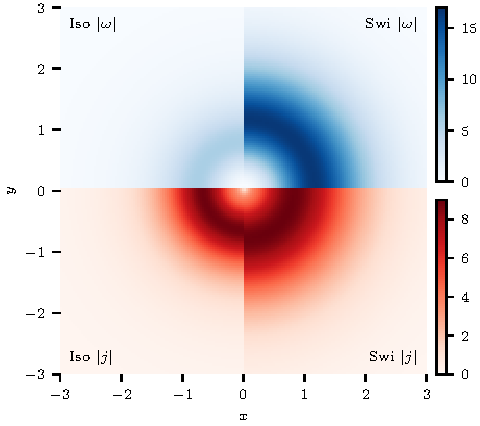
\includegraphics[width=\linewidth]{v-4r-4_vorticity_current_ring_t_3}
      \caption{Vorticity and current density rings at $t=3$. The switching model permits rings of greater radial extent and notably stronger current density.}
      \label{fig:v-4r-4_vorticity_current_ring_t_3}
    \end{subfigure}
\caption{Kinetic energy as a function of time, and the vorticity and current density rings at $t=3$.}
\label{fig:ke_and_rings}%
\end{figure}

Initially, at $t=1$ the torsional Alfv\'en waves injected by the driver trace the field surrounding the null, moving towards the fan plane and out from the spine. The waves eventually meet and create an shear layer in the velocity and magnetic field in the form of a ring of vorticity and current density. Without any diffusion in the system the main wavefronts would travel far along the field before meeting. The presence of both viscosity and resistivity encourages the waves to diffuse as they travel along the field, allowing the upper and lower waves to meet relatively close to the spine, creating rings of shear which are both thicker and smaller in radius. In the switching case, due to the switching model diffusing the field less effectively than the isotropic model, the rings are larger in radius, stronger in magnitude, and thinner (Figure~\ref{fig:v-4r-4_vorticity_current_ring_t_3}). Since the viscosity diffuses velocity directly and affects the magnetic field only indirectly, the vorticity is affected by the change in viscosity model more than the current density.

\begin{figure}[t]
  \centering
    \begin{subfigure}{0.32\textwidth}
      \includegraphics[width=\linewidth]{v-4r-4_uz_t_2}
      \caption{$t=2$}
      \label{fig:v-4r-4_uz_t_2}
    \end{subfigure}
    \begin{subfigure}{0.32\textwidth}
      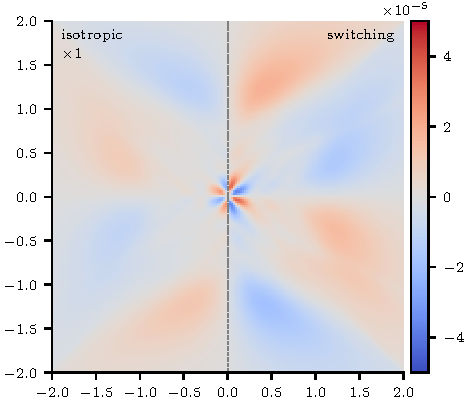
\includegraphics[width=\linewidth]{v-4r-4_uz_t_4}
      \caption{$t=4$}
      \label{fig:v-4r-4_uz_t_4}
    \end{subfigure}
    \begin{subfigure}{0.32\textwidth}
      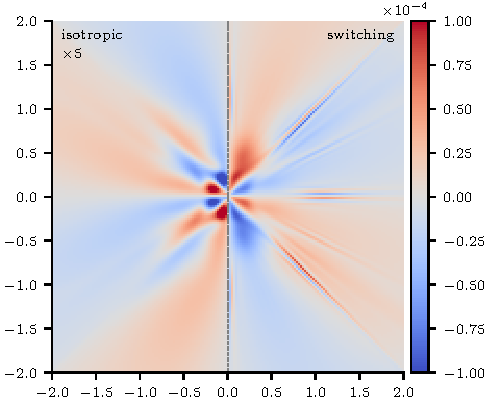
\includegraphics[width=\linewidth]{v-4r-4_uz_t_6}
      \caption{$t=6$}
      \label{fig:v-4r-4_uz_t_6}
    \end{subfigure}
    \begin{subfigure}{0.32\textwidth}
      \includegraphics[width=\linewidth]{v-4r-4_uz_t_8}
      \caption{$t=8$}
      \label{fig:v-4r-4_uz_t_8}
    \end{subfigure}
    \begin{subfigure}{0.32\textwidth}
      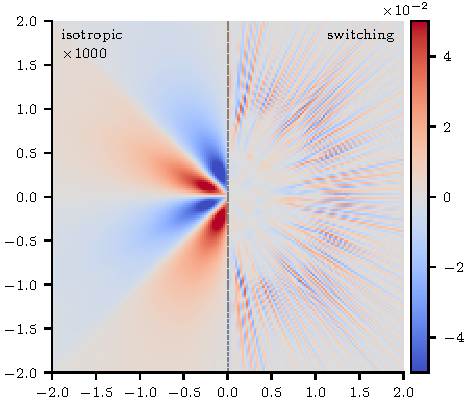
\includegraphics[width=\linewidth]{v-4r-4_uz_t_10}
      \caption{$t=10$}
      \label{fig:v-4r-4_uz_t_10}
    \end{subfigure}
    \begin{subfigure}{0.32\textwidth}
      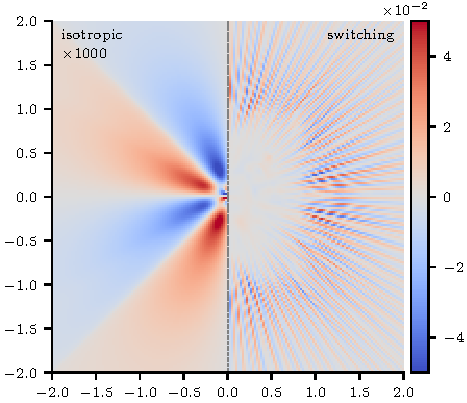
\includegraphics[width=\linewidth]{v-4r-4_uz_t_12}
      \caption{$t=12$}
      \label{fig:v-4r-4_uz_t_12}
    \end{subfigure}
\caption{Out of plane velocity at $t=2, 4, 6, 8, 10$ and $12$ for both viscosity models (isotropic on the left of each image, switching on the right). Note the isotropic results have been multiplied by as much as $1000$ in order to compare to the switching results. In the switching case an initial perturbation appears at $t=2$ and grows in amplitude as well as spreading radially, initially along the diagonals, before extending azimuthally. In the isotropic case there is no evidence of the KHI, however at $t=12$ there is evidence of what we find to be a form of fluting instability.}
\label{fig:out_of_place_velocity}%
\end{figure}

\todo{field lines after KHI}

In the switching case, the velocity shear layer becomes unstable to the KHI, initially presenting as a low-amplitude perturbation overlaying the initial velocity structure. This structure appears to be associated with boundary effects (Figure~\ref{fig:v-4r-4_uz_t_2}) and is very similar comparing the two cases. The initial perturbation extends from $r\approx0.3$ to $r\approx1$. As it grows in amplitude, it spreads outwards in the fan plane, initially along the diagonals (Figure~\ref{fig:v-4r-4_uz_t_8}) before spreading azimuthally (Figure~\ref{fig:v-4r-4_uz_t_12}). The joint effect of radial spreading and perturbation growth gives rise to the specific shape of the growth in kinetic energy with time (Figure~\ref{fig:v-4r-4_kinetic_energy}). There is no evidence of the KHI in the isotropic case, however, starting from $t=8$ there is evidence of a change in behaviour very near the null, eventually creating what appear as plume-like structures at $t=12$. As shall be discussed further on, this is the initial appearance of the fluting instability.

\begin{figure}[t]
  \centering
    \begin{subfigure}{0.49\textwidth}
      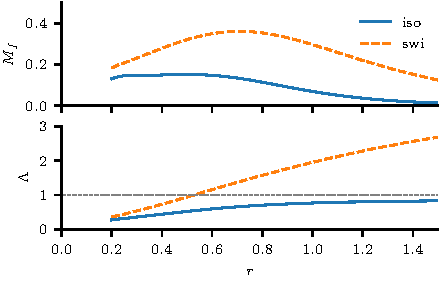
\includegraphics[width=\linewidth]{v-4r-4_mach_t_6}
      \caption{}%
      \label{fig:v-4r-4_mach_t_6}
    \end{subfigure}
    \hfill
    \begin{subfigure}{0.49\textwidth}
      \includegraphics[width=\linewidth]{v-4r-4_layers_with_time}
      \caption{}
      \label{fig:v-4r-4_layers_with_time}
    \end{subfigure}
\caption{Properties of the shear layers for the isotropic case (blue, solid line) and switching case (orange, dashed line). On the left is a plot of the fast Mach number $M_f$ and stability measure $\Lambda$ as functions of radius $r$ at $t=6$. The measure $\Lambda$ confirms that the current-vortex sheet in the isotropic case is linearly stable to the KHI and unstable in the switching case for $r>0.5$. In the switching case the peak of $M_f$ aligns with the observed region of high growth of the instability. On the right is the dependence of the shear widths $L_u$ and $L_B$ and the shear magnitudes $\Delta u$ and $\Delta B$ as functions of time and at a radius of $r=0.7$. Both magnetic and velocity shear layers are notably thinner and the velocity shear is notably stronger in the switching case. The strength of the magnetic shear at this radius is decreased by the use of the switching model.}
\label{fig:v-4r-4_layers}%
\end{figure}

Figure~\ref{fig:v-4r-4_mach_t_6} shows the relevant stability measures as functions of radius across the fan plane at $t=6$, a time when the KHI is notably unstable in the switching case and stable in the isotropic case. The stability measures show that the use of isotropic viscosity results in shear layers that are stable to the KHI, as observed. This is in contrast to the less diffusive switching viscosity which permits KHI-unstable shear layers. Figure~\ref{fig:v-4r-4_layers_with_time} shows that the main effect of the switching model is to massively increase the magnitude of the velocity shear. It is this effect that increases both $M_f$ and $\Lambda$ and encourages shear layers which are unstable to the KHI.

\begin{figure}[t]
  \centering
    \begin{subfigure}{0.49\textwidth}
      \includegraphics[width=\linewidth]{v-4r-4_counterflows_t_3}
      \caption{Azimuthal velocity}
      \label{fig:v-4r-4_counterflows_t_3}
    \end{subfigure}
    \hfill
    \begin{subfigure}{0.49\textwidth}
      \includegraphics[width=\linewidth]{v-4r-4_lorentz_counterflows_t_3}
      \caption{Azimuthal component of Lorentz force}
      \label{fig:v-4r-4_lorentz_counterflows_t_3}
    \end{subfigure}
\caption{Azimuthal flows counter to the relevant driver are accelerated due to the action of the magnetic tension force. Both figures are sliced through $x$ and show both isotropic (left of each image) and switching (right of each image) results.}
\label{fig:counterflows}%
\end{figure}

Due to the field attempting to straighten the twist introduced by the driver, magnetic tension close to the spine opposes the direction of the twisting motion and causes counterflows to appear (Figure~\ref{fig:counterflows}). These counterflows play a part in the fluting instability found at a later time and could, with a suitable parameter choice, generate their own KHI. We do not investigate the potential for a secondary KHI further due to constraints on the numerical resolution of the simulations. This is a valid avenue of further study however, since such an instability close to the null could play a notable part in reconnection there.

\begin{figure}[t]
  \centering
    \begin{subfigure}{0.48\textwidth}
      \includegraphics[width=\linewidth]{v-4r-4_vorticity_current_ring_t_10}
      \caption{Current-vortex sheet at $t=10$ (top left is multiplied by 10)}
      \label{fig:v-4r-4_vorticity_current_ring_t_10}
    \end{subfigure}
    \hfill
    \begin{subfigure}{0.48\textwidth}
      \includegraphics[width=\linewidth]{v-4r-4_reconn_rate_t_10}
      \caption{A sample of field-line integrations of the parallel electric field at $t=10$ for both viscosity models. Field lines have been integrated from near the upper $z$-boundary at $z=0.23$ to where they meet any other boundary. The pattern of enhanced reconnection associated with the KHI is visible in the switching case.}
      \label{fig:v-4r-4_reconn_rate_t_10}
    \end{subfigure}
\caption{The current-vortex sheet and spatial distribution of the reconnection rate at $t=10$.}
\end{figure}

In both cases the current-vortex sheet grows in radius and magnitude, more in the switching case than in the isotropic, although the shearing action of the counterflows has produced a secondary ring of strong current density closer to the spine which is greater in magnitude in the isotropic case. By $t=10$ the KHI has disrupted the current-vortex sheet (Figure~\ref{fig:v-4r-4_vorticity_current_ring_t_10}) and the resultant rolls of the KHI create strong current sheets, enhancing the local reconnection rate. Figure~\ref{fig:v-4r-4_reconn_rate_t_10} shows the pattern of enhanced reconnection in the switching case, visibly similar to the pattern in the current density itself, but incorporating the twist of the integrated field line.

\begin{figure}[t]
  \centering
  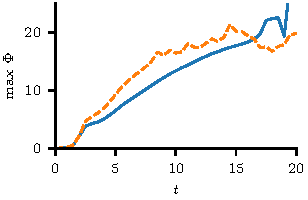
\includegraphics[width=0.5\linewidth]{v-4r-4_reconn_rate_over_time}
  \caption{Reconnection rate over time. Both isotropic (blue, solid line) and switching (orange, dashed line) models are shown. As twist is injected by the drivers over time, the reconnection rate increases, more in the switching case due to the reconnection-enhancing effect of the KHI.}%
  \label{fig:v-4r-4_reconn_rate_over_time}
\end{figure}

While the enhanced reconnection in the fan plane caused by the KHI is of interest, the maximum reconnection rate actually occurs very close to the spine (Figure~\ref{fig:v-4r-4_reconn_rate_t_10}) and is notably greater in the switching case. This slippage reconnection is more efficient in the switching case due to the switching viscosity allowing much thinner, stronger current structures to evolve. Figure~\ref{fig:v-4r-4_reconn_rate_over_time} shows the peak reconnection rate in both cases as functions of time, clearly showing more efficient reconnection in the switching case.

\subsubsection{Spine-fan reconnection}

\begin{figure}[t]
  \centering
    \begin{subfigure}{0.32\textwidth}
      \includegraphics[width=\linewidth]{v-4r-4-spine-fan-reconn-34.pdf}
      \caption{$t=17$}
      \label{fig:v-4r-4-spine-fan-reconn-34}
    \end{subfigure}
    \hfill
    \begin{subfigure}{0.32\textwidth}
      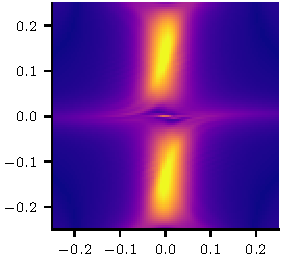
\includegraphics[width=\linewidth]{v-4r-4-spine-fan-reconn-35.pdf}
      \caption{$t=17.5$}
      \label{fig:v-4r-4-spine-fan-reconn-35}
    \end{subfigure}
    \hfill
    \begin{subfigure}{0.32\textwidth}
      \includegraphics[width=\linewidth]{v-4r-4-spine-fan-reconn-36.pdf}
      \caption{$t=18$}
      \label{fig:v-4r-4-spine-fan-reconn-36}
    \end{subfigure}
\caption{Development of the spine-fan reconnection current sheet shown as plots of $|\vec{j}|$ sliced through $y=0$ between $t=17$ and $18$. Maximum current density in all plots is $|\vec{j}| = 120$.}
\label{fig:spine_fan_reconnection_current_sheet}
\end{figure}

In typical studies of spine-fan reconnection (such as~\cite{pontinCurrentSheetFormation2007}) the spines of a null point are dragged in opposite directions at the boundaries. Once the disturbances have travelled along the spines, they meet at the null and create a current sheet which acts to reconnect field lines between a spine and its associated fan. Here, the spines are not dragged at their foot points but are shifted near where they meet the fan plane in the following way.

The twist in the spines creates a current which heats the contained plasma and generates a small pressure gradient towards the null point, driving two oppositely directed streams of plasma above and below the null (figure~\todo{vz plots}). When these streams meet at the null point, they form a stagnation flow, compressing the plasma in the vicinity of the null and flowing out along the fan plane. If the streams are not symmetrical, that is one is slightly deflected, then the resulting imbalance in momentum will cause both streams to deflect in opposite directions. This imbalance in the velocity is found at time $t=TODO$ (figure~\todo{vz imbalance}). The flow along the fan plane becomes asymmetric as a result (figure~\todo{vx imbalance}) which encourages the gradual movement of the spines in opposing directions.

\begin{figure}[t]
  \centering
    \begin{subfigure}{0.49\textwidth}
      \includegraphics[width=\linewidth]{field_line_plots/cropped/v-4r-4-isotropic_0030_cropped.png}
      \caption{$t=15$}
      \label{fig:v-4r-4-iso-field-30}
    \end{subfigure}
    \hfill
    \begin{subfigure}{0.49\textwidth}
      \includegraphics[width=\linewidth]{field_line_plots/cropped/v-4r-4-isotropic_0037_cropped.png}
      \caption{$t=18.5$}
      \label{fig:v-4r-4-iso-field-37}
    \end{subfigure}
\caption{Collapse of the null point visualised with field lines. Field lines are plotted from a circle of radius $0.05$ around the upper and lower spine footpoints. Contours of $|\vec{j}| = 60$ are also plotted and reveal the strong current within the spine as well as the formation of the central sheet associated with the spine-fan reconnection. At $t=18.5$ the bulk of the field lines making up the core of the spines have reconnected.}
\label{fig:khi_field_lines_collapse}
\end{figure}

This movement of the magnetic field near the null creates a current sheet though the null point itself which enables reconnection between the spine and the opposite fan (figures~\ref{fig:spine_fan_reconnection_current_sheet} and~\ref{fig:v-4r-4-iso-field-37}). The development of the current sheet and the resultant spine-fan reconnection is similar to that of~\cite{pontinCurrentSheetFormation2007} with the exception that the twist in the field begins to unravel as the reconnection proceeds. 

\subsection{Analysis of parameter study}

The results shown in section~\ref{sec:null_point_khi_single_case} do not dramatically change when the viscosity $\nu$ is varied. However, the value of $\eta$ has a strong impact on the dynamics of the stressed null. Generally, increasing $\eta$ to $10^{-3}$ produces a null that remains unstable to the KHI (when using switching viscosity) but shows no sign of collapse. In contrast, decreasing $\eta$ to $10^{-5}$ causes the null to collapse much sooner than in the example case in section~\ref{sec:null_point_khi_single_case}, so much so that the KHI doesn't have time to develop nonlinearly, even in linearly unstable cases. We present first the quantitative effect of varying $\nu$, $\eta$ and the viscosity models on the properties of the shear layers and the resulting stability and development of the KHI. We then focus our analysis on the effect of only $\eta$ on the fluting instability and the null collapse, still comparing the two viscosity models.

%As an aside, in all $\nu = 10^{-3}$ isotropic simulations there's an unexpected, transient artifact in every examined variable. This was also seen in the kink instability simulations in chapter TODO. This is assumed to be due to small-amplitude fast waves created during the initial ramp up, the interaction of which causes the isotropic viscous stress tensor to produce odd effects. It appears to only affect the first time step and the effect is only to slightly increase the viscous heating. Since the affected results don't differ wildly from those of the unaffected $\nu=10^{-4}$ simulations we cautiously trust these results.

\subsubsection{Shear layer properties and instability}

To understand the effect that viscosity and resistivity have on the stability of the current-vortex sheet, it is useful to understand how changing their strength affects the thickness and magnitude of the vorticity and current density rings. After presenting an analysis of how these shear layer properties change with $\nu$ and $\eta$, the stability of these layers is presented and compared to predictions from the theoretical measures of stability introduced in section~\ref{sec:stability_measures}. The overall effect of viscosity and resistivity is to diffuse the upper and lower Alfv\'en waves as they travel through the null before meeting and diffusing in the fan plane, forming the shear layers that make up the current-vortex sheet. 

\begin{figure}[h]
  \centering
  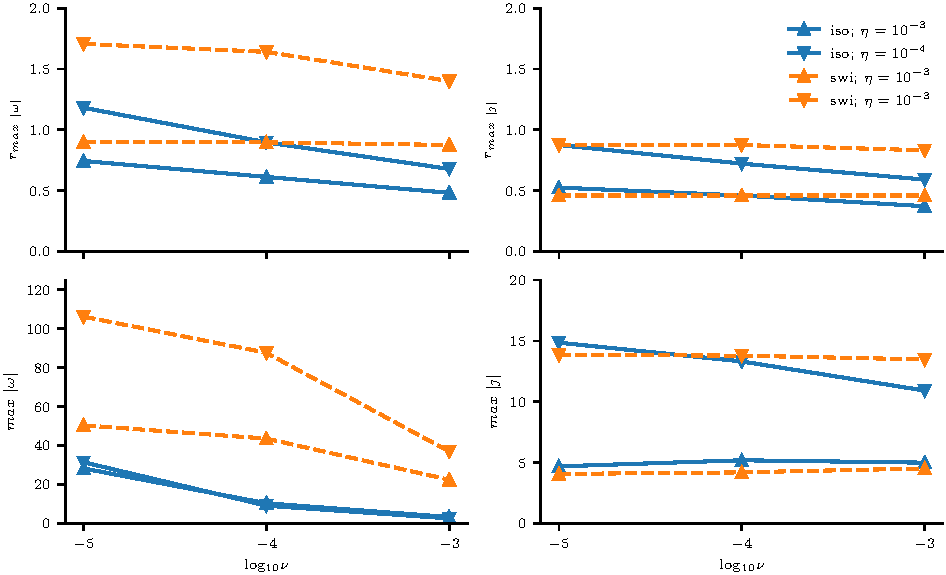
\includegraphics[width=\linewidth]{param_study/peak_mag_and_loc.pdf}
  \caption{Peak vorticity and current and the radii at which the peaks occur as functions of $\nu$ for each value of $\eta$ at $t=8$. The symbols represent $\eta=10^{-3}$ (downward-facing triangle) and $\eta=10^{-4}$ (upward-facing triangle) and the line styles represent the form of viscosity used, either isotropic (blue, solid lines) or switching (orange, dashed lines). In the isotropic case, both rings decrease in radial extent as either diffusion parameter is increased. In the switching case, both rings also decrease with $\eta$, however there is a notable increase in the radial extent with $\nu$, particularly for high values of $\eta$.}%
  \label{fig:param_study_peak_mag_and_loc}
\end{figure}

Figure~\ref{fig:param_study_peak_mag_and_loc} presents the peak vorticity and current density as functions of $\nu$ for both values of $\eta$, also plotting the radii at which the peaks occur. Increased diffusion leads to a thicker, weaker ring with a smaller radius. This is reflected in the general trends found in figure~\ref{fig:param_study_peak_mag_and_loc}, where peak current, peak vorticity and the radii at which the peaks occur all decrease with both diffusion parameters. The switching model, being generally less diffusive than the isotropic model, permits velocity shear layers with much greater peak vorticity and radial extent. Due to the coupling between the magnetic field and the velocity in an Alfv\'en wave, the isotropic model appears to provide some diffusion to the magnetic field during the formation of the magnetic shear layer, resulting in a layer with weaker peak current and smaller radial extent, however the switching model affects the layer very little.

\begin{figure}[t]
  \centering
  \includegraphics[width=1.0\linewidth]{param_study/layer_thickness_and_shear.pdf}
  \caption{The thickness of the velocity and magnetic shear layers $L_u$ and $L_B$, respectively, and the difference in velocity $\Delta u$ and magnetic field $\Delta B$ across the layers as functions of $\nu$ for each value of $\eta$ at $t=8$. The values for the velocity and magnetic shear layers are calculated at the radius at which the peak vorticity and current density occur, respectively. Increased diffusion in the form of either resistivity or viscosity results in thicker shear layers. As $\nu$ increases $\Delta u$ decreases and $\Delta B$ increases.}%
  \label{fig:layer_thickness_and_shear}
\end{figure}

Figure~\ref{fig:layer_thickness_and_shear} presents a measure of the thickness, $L_u$ and $L_B$, and the magnitudes, $\Delta u$ and $\Delta B$, of the velocity and magnetic shear layers, respectively. The radius at which these values are measured is the radius at which the peak vorticity or current density is found (as reported in figure~\ref{fig:param_study_peak_mag_and_loc}). 

The thickness of the shear layers is a direct result of how the initial Alfv\'en waves diffuse as they travel towards the fan plane. As the diffusion in the system increases, the thickness of the shear layers increases correspondingly (figure~\ref{fig:layer_thickness_and_shear}). Since the switching model is less diffusive than the isotropic model, the shear layers are generally thinner using this model. The effect of viscosity on the differences of velocity and magnetic field across the shear layers is more complex. With increased viscous diffusion, velocity is diffused more efficiently and the velocity difference across the velocity shear layer is reduced. In contrast, with increased viscous diffusion, the magnetic field difference across the magnetic shear layer is increased. This is a direct result of the enhanced viscous diffusion causing the initial Alfv\'en waves to meet closer to the null.

The distance the Alfv\'en waves travel before meeting affects the magnetic shear layer in two ways. Firstly, when the Alfv\'en waves are allowed to travel far along the field before forming the shear layers, the magnetic field on either side of the shear has more time to diffuse and reduce in magnitude. The other effect is a little more involved. Consider the effect of sending a wave pulse along a cable. Without much tension in the cable, the pulse has a certain amplitude. With greater tension in the cable, the energy required to bend the cable is increased, so the same pulse (with the same energy) will not be able to bend the cable quite so much and the resultant wave will have a smaller amplitude. Since the magnetic field strength of this particular null increases linearly with distance from the origin, the magnetic tension increases too. Analogous to the wave travelling along a cable under higher-tension, the Alfv\'en wave which travels further along the increasing magnetic field will be reduced in amplitude, hence reducing the magnitude of the magnetic shear.

\begin{figure}[h]
  \centering
  
\includegraphics[width=\linewidth]{param_study/kinetic_energies.pdf}
  \caption{Kinetic energy against time for each parameter choice. Runs using isotropic viscosity are shown as blue (solid) lines and switching viscosity as orange (dashed) lines. The distinctive energy profile of the Kelvin-Helmholtz instability is apparent in all switching cases and in the single isotropic case corresponding to $\nu = 10^{-5}, \eta = 10^{-3}$ in subfigure (a). Reconnection associated with the collapse of the null is signalled by sharp spikes in the kinetic energy starting around $t\approx13$ in the $\eta = 10^{-4}$ cases, subfigures (d-f), particularly in the isotropic cases. An increase in $\nu$ damps the energy released during the KHI in the switching cases and totally suppresses the KHI in the isotropic cases.}%
  \label{fig:param_study_kinetic_energies}
\end{figure}

The observed stability of KHI in the fan plane is determined via inspection of the out of plane velocity for each parameter choice and is summarised for each parameter choice in table~\ref{tab:stability}. The velocity is inspected at $t=8$, before the onset of other phenomena such as the null collapse. The stability and nonlinear development is also reflected in the kinetic energies~\ref{fig:param_study_kinetic_energies}. Simulations using the switching model develop a kinetic energy profile which displays a growth and decay shape indicative of the KHI. A similar pattern is also seen in the single fully-unstable isotropic case, figure~\ref{fig:param_study_kinetic_energies}(a).

The kinetic energy profiles also reveal some interesting cases of marginal stability which are investigated further by inspecting the out of plane velocity for $t>8$. The isotropic case~\ref{fig:param_study_kinetic_energies}(b) is found to be stable at all times, yet shows KHI-like growth in the kinetic energy. The isotropic case~\ref{fig:param_study_kinetic_energies}(d) and the switching case~\ref{fig:param_study_kinetic_energies}(f) show similar kinetic energy profiles and, upon inspection, show signs of instability at $t=12$. The full development of the instability in both cases is interrupted by the collapse of the null.

\begin{table}[]
\centering
\begin{tabular}{llllll}
$\nu$    & $\eta$    & $Pr_m = \nu/\eta$ & Isotropic stability & Switching stability &  \\
\midrule
$10^{-3}$ & $10^{-3}$ & $1$ & Stable                 & Unstable                 &  \\
$10^{-4}$ & $10^{-3}$ & $0.1$ & Stable                 & Unstable                 &  \\
$10^{-5}$ & $10^{-3}$ & $0.01$ & Unstable                 & Unstable                 &  \\
$10^{-3}$ & $10^{-4}$ & $10$ & Stable                 & Marginally unstable                 &  \\
$10^{-4}$ & $10^{-4}$ & $1$ & Stable                 & Unstable                 &  \\
$10^{-5}$ & $10^{-4}$ & $0.1$ & Marginally unstable                 & Unstable                 & 
\end{tabular}
\caption{Stability in the isotopic and switching cases for different choices of $\nu$ and $\eta$. The magnetic Prandtl number Pr$_m$ is also stated. The isotropic model mostly results in stability while the switching model mostly results in instability. There are two marginally unstable cases where the instability does not have time to fully develop.}
\label{tab:stability}
\end{table}

To further explore the observed stability of the KHI, we investigate how $M_f$ and $\Lambda$ vary radially, and link this to the stability and growth of the KHI. As an indicator of the stability of the shear layer, we plot the Mach number associated with the fast-mode $M_f = \frac{\Delta u}{\sqrt{c_s^2 + c_A^2}}$, where $\Delta u$ is the difference in velocity over the shear layer, and $c_s$ and $c_A$ are the local sound and Alfv\'en speeds, respectively, as well as the parameter $\Lambda = \frac{L_B}{L_u}(M_{A, proj})^{2/3}$, where $L_B$ and $L_u$ are the widths of the respective magnetic and velocity shear layers, and $M_{A, proj}$ is the Alfv\'en velocity of the layer after removing the guide field, i.e. $M_{A, proj} = \frac{\Delta u \sqrt{\rho}}{\Delta B}$ (TODO reword this entire sentence). For the layer to be theoretically unstable to the KHI, $M_f < 2$ and $\Lambda > 1$. These properties are investigated at $t=8$, around the time of KHI onset where it occurs, but well before the breakup of the current-vortex sheet, allowing accurate measurement of $M_f$ and $\Lambda$.

\begin{figure}[h]
    \hfill
    \begin{subfigure}{0.49\textwidth}
      \centering
  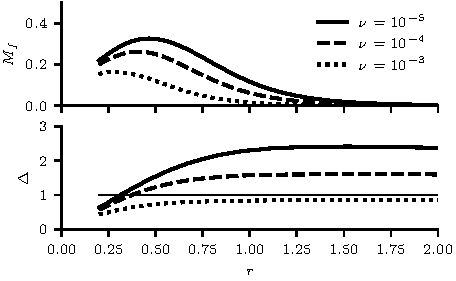
\includegraphics[width=1.0\linewidth]{param_study/mach_numbers_eta_3_iso.pdf}
      \caption{Isotropic; $\eta = 10^{-3}$}%
      \label{fig:mach_numbers_eta_3_iso}
    \end{subfigure}
    \hfill
    \begin{subfigure}{0.49\textwidth}
      \centering
  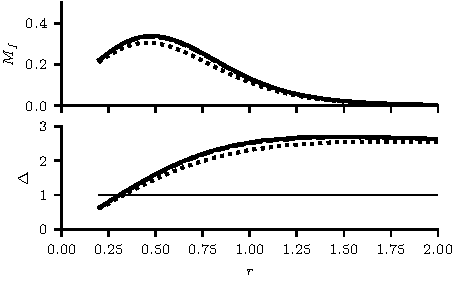
\includegraphics[width=1.0\linewidth]{param_study/mach_numbers_eta_3_swi.pdf}
      \caption{Switching; $\eta = 10^{-3}$}%
      \label{fig:mach_numbers_eta_3_swi}
    \end{subfigure}
    \hfill
    \begin{subfigure}{0.49\textwidth}
      \centering
  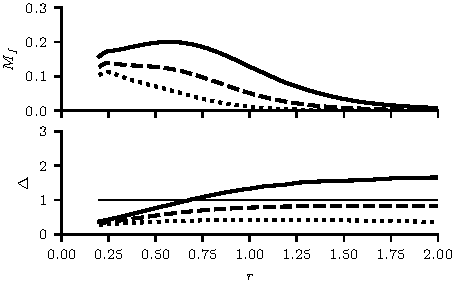
\includegraphics[width=1.0\linewidth]{param_study/mach_numbers_eta_4_iso.pdf}
      \caption{Isotropic; $\eta = 10^{-4}$}%
      \label{fig:mach_numbers_eta_4_iso}
    \end{subfigure}
    \hfill
    \begin{subfigure}{0.49\textwidth}
      \centering
  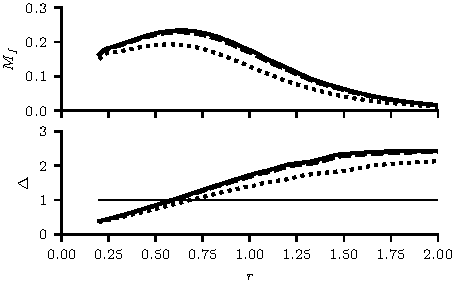
\includegraphics[width=1.0\linewidth]{param_study/mach_numbers_eta_4_swi.pdf}
      \caption{Switching; $\eta = 10^{-4}$}%
      \label{fig:mach_numbers_eta_4_swi}
    \end{subfigure}

  \caption{Plots of $M_f$ and $\Lambda$ as functions of $r$ for all parameter choices at $t=8$. Note the difference in the scale of $M_f$ for difference values of $\eta$. The cases where $\Lambda > 1$ are unstable with the exception of the isotropic cases where $\nu=10^{-4},\eta=10^{-3}$ (dashed line in figure~\ref{fig:mach_numbers_eta_3_iso}).}%
  \label{fig:mach_numbers}
\end{figure}

The observed stability summarised in table~\ref{tab:stability} is well matched by the theoretical conditions of instability, $\Lambda > 1$ and $M_f < 2$. Figure\ref{fig:mach_numbers} shows $M_f$ and $\Lambda$ plotted as functions of $r$ for each parameter choice. The condition $M_f < 2$ is satisfied in all runs, however the location of the peak of $M_f$ is where the current-vortex sheet is most unstable. Over all parameters, the maximum value of $M_f$ is less than $0.5$ suggesting the system would have to be driven at an unrealistically high velocity to approach the limit of $2$. The pertinent condition of instability for this particular presentation of the instability is thus $\Lambda > 1$. The simulations where this conditions is satisfied are unstable in all by one case, indicating that despite the difference in geometry and physics, the stability analysis of~\cite{einaudiResistiveInstabilitiesFlowing1986} is of practical use in predicting the stability of the KHI in magnetic null points. This condition even accurately predicts the stability of the marginal cases discussed previously. 

The isotropic case where $\nu=10^{-4},\eta=10^{-3}$ (dashed line in figure~\ref{fig:mach_numbers_eta_3_iso}) is the one outlier case where $\Lambda > 1$ over much of the current-vortex sheet, yet no instability is found in the out of plane velocity. The associated kinetic energy, figure~\ref{fig:param_study_kinetic_energies}(b), does show some initial growth, however this plateaus around $t\approx7.5$ and shows no further increase, unlike the kinetic energy of the marginally unstable isotropic case, figure~\ref{fig:param_study_kinetic_energies}(d), which continues to slowly increase. This suggests that the viscosity can affect stability not only by changing the thickness and magnitude of the current-vortex sheet as it forms, but also by stabilising a sheet which would otherwise be unstable. 

\begin{figure}[t]
  \centering
  \includegraphics[width=1.0\linewidth]{param_study/reconnection_rate.pdf}
  \caption{The reconnection rate max$\Phi$ as a function of time for each parameter choice. In all cases the reconnection rate increases with time due to slippage reconnection occurring throughout the null and within the magnetic shear layer. Where the KHI is excited, it encourages a greater rate of reconnection and causes the rate to temporarily dip around $t=10$, except in one case (subfigure (e)). Where $\eta=10^{-4}$ the isotropic cases show evidence of the reconnection rate dipping when the null collapses and the reconnecting current structures are disrupted, around $t=14$.}%
  \label{fig:khi_param_study_reconnection_rate}
\end{figure}

Figure~\ref{fig:khi_param_study_reconnection_rate} shows the reconnection rate over time for each parameter choice. Generally the switching model enhances the reconnection rate. This is due to the enhanced reconnection caused by the KHI, shown by the fact that the single fully-unstable isotropic case shares a similar reconnection rate profile (figure~\ref{fig:khi_param_study_reconnection_rate}(a)). When the KHI goes fully unstable, around $t=10$, the reconnection rate dips, except in the case of figure~\ref{fig:khi_param_study_reconnection_rate}(e) where the reconnection rate is significantly, transiently enhanced. The dip in reconnection rate coincides with a dip in kinetic energy (figure~\ref{fig:param_study_kinetic_energies}), indicating this is the point at which the KHI fully disrupts the current-vortex sheet, stalling the growth of the KHI and reducing the slippage reconnection which was occurring within the current ring. The case of the increase in reconnection rate in figure~\ref{fig:khi_param_study_reconnection_rate}(e) can be explained by noting that the break up of the current-vortex sheet is likely somewhat turbulent and could create transient current sheets capable of a high reconnection rate. The reconnection rate may be temporally under-resolved in this case. In the isotropic cases where $\eta=10^{-4}$ (figures~\ref{fig:khi_param_study_reconnection_rate}(d-f)) the collapse of the null is revealed in the reconnection rate, where the rate begins to dip at $t=14$.

Just as is found in the single case shown in section~\ref{sec:null_point_khi_single_case}, the simulations where $\eta = 10^{-4}$ show signs of collapse of the null starting around $t=13$, indicated by a sudden, bursty increase in kinetic energy~\ref{fig:param_study_kinetic_energies}(a-c), and the dip in the reconnection rate (figures~\ref{fig:khi_param_study_reconnection_rate}(d-f)) at $t=14$. The reason this occurs earlier in the parameter study simulations than in the higher resolution case in section~\ref{sec:null_point_khi_single_case} is because the lower resolution results in current structures compressing to the grid scale sooner, thereby setting off fast reconnection at an earlier time. 

\subsection{Summary of results and conclusions}

In this chapter I have compared two models of viscosity applied to a magnetic null point which has been dynamically twisted at its footpoints in such a way that a current-vortex sheet forms in the fan plane. This sheet has the potential to become unstable to the KHI. It was found that increased viscous dissipation has a stabilising effect on the sheet, especially when the isotropic model is employed. This is due to viscosity thickening the sheet, increasing its stability. The presence of the instability enhances reconnection locally within the sheet.

This numerical experiment has also shown that a null point can spontaneously collapse when subjected to a high degree of twist in its spines. The collapse is driven by spine-fan reconnection and its development is strongly influenced by the unravelling of the twisted spines. This may have an effect on the null's ability to undergo oscillatory reconnection (see~\cite{thurgoodThreedimensionalOscillatoryMagnetic2017}).

What are consequences \& implications of results?

What are downsides?

TODO

In hindsight, the resolution could have been better balanced by using more grid points in the relatively long $x$ and $y$ directions than the relatively short $z$ direction. A non-uniform grid could have been used, with higher resolution focused near the null point. We believe this would have sped up the runtime of the simulations and provided slightly better quantitative results, particularly for the simulations using low values for the resistivity and viscosity. however the results as presented have been verified with higher resolution tests of a sample of simulations. These were performed at double the resolution of $640$ grid points per dimension. .
